\documentclass{article}

\usepackage{listings}
\usepackage{graphicx}
\usepackage{float}
\usepackage{amsmath}
\usepackage{geometry}
 \geometry{
 a4paper,
 total={170mm,257mm},
 left=20mm,
 top=20mm,
 }

\author{David Kolden, davidko}
\title{Mandatory assignment 1: Traveling Salesman Problem}

\begin{document}

\maketitle
\tableofcontents

\section{Introduction}
Brief explanation of the assignment, how to start the programs
\section{Exhaustive search}

Start the program with
\begin{lstlisting}[language=bash]
	$ python3 exhaustive.py european_cities.csv 
\end{lstlisting}
The program will find the shortest tour between 6 - 10 cities. The program outputs

\begin{lstlisting}[language=bash]
For n_cities = 6:
Best distance: 5018.8099999999995
Best sequence: (0, 1, 4, 5, 2, 3)
Best order of travel: Barcelona Belgrade Bucharest Budapest Berlin 
Brussels Barcelona
 
For n_cities = 7:
Best distance: 5487.889999999999
Best sequence: (2, 6, 3, 0, 1, 4, 5)
Best order of travel: Berlin Copenhagen Brussels Barcelona Belgrade 
Bucharest Budapest Berlin
 
For n_cities = 8:
Best distance: 6667.489999999999
Best sequence: (3, 7, 0, 1, 4, 5, 2, 6)
Best order of travel: Brussels Dublin Barcelona Belgrade Bucharest 
Budapest Berlin Copenhagen Brussels
 
For n_cities = 9:
Best distance: 6678.549999999999
Best sequence: (2, 6, 8, 3, 7, 0, 1, 4, 5)
Best order of travel: Berlin Copenhagen Hamburg Brussels Dublin 
Barcelona Belgrade Bucharest Budapest Berlin
 
For n_cities = 10:
Best distance: 7486.309999999999
Best sequence: (6, 8, 3, 7, 0, 1, 9, 4, 5, 2)
Best order of travel: Copenhagen Hamburg Brussels Dublin Barcelona 
Belgrade Istanbul Bucharest Budapest Berlin Copenhagen
	 
Time spent[seconds]: [0.002037, 0.015967, 0.134317, 1.310069, 
13.964733]
\end{lstlisting}

The time used by the algorithm to find the best distance was measured. The time spent on solving TSP for six, seven, eight, nine and ten cities is shown in the last two lines of the program output and in figure 1.

\begin{figure}[H]
\begin{center}
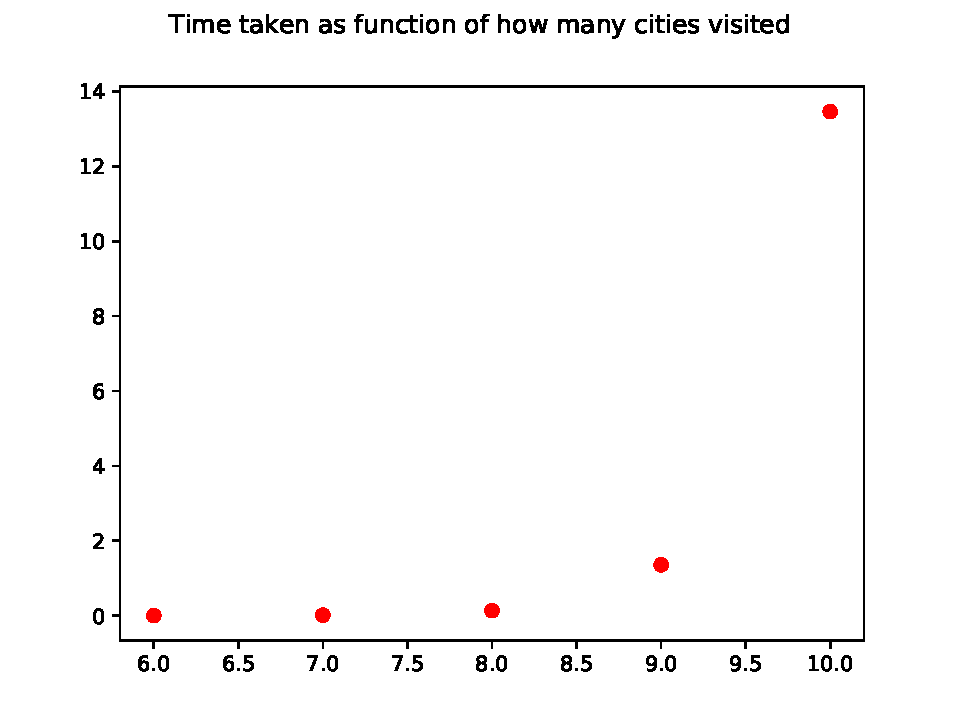
\includegraphics[scale=0.8]{"../Exhaustive.pdf}
\caption{Time spent for the TSP algorithm}
\end{center}
\end{figure}

It can be seen that the time spent by the algorithm searching the TSP for \textit{n} cities is roughly the time spent on calculating with \textit{n-1} cities multiplied by \textit{n}. The time spent by the algorithm to search TSP for 24 cities can be calculated with
\[
	t_{10} \frac{24!}{10!} \approx 14s \cdot \frac{24!}{10!} \approx 2.4 \cdot 10^{18}
\]


\section{Hill Climbing}

Start the program with
\begin{lstlisting}[language=bash]
	$ python3 hill_climber.py european_cities.csv 
\end{lstlisting}
Compare with exhaustive for 10 cities, run algorithm 20 times, report best worst mean and standard deviation for 10 runs and 24 runs
\begin{lstlisting}[language=bash]
For 10 cities:
Best distance: 7486.309999999999
Worst distance: 8352.7
Average distance: 7749.23
Standard deviation: 227.292
 
For 24 cities:
Best distance: 20129.510000000002
Worst distance: 22330.250000000004
Average distance: 21573.8
Standard deviation: 456.155
\end{lstlisting}

\section{Genetic algorithm}
Report parameters used, report best worst mean and deviation of 20 runs with three different values for population size, plot of average fitness of best individual of each run
\begin{lstlisting}[language=bash]
Search: 24 cities, population size: 10, number of generations: 500, 
number of rounds: 20, number of children: 4: 
Best distance: 13783.62
Worst distance: 17690.740000000005
Average distance: 16147.2
Standard deviation: 1044.07
Time [seconds]: 3.745909
Best order of travel: 
Munich Vienna Kiev Stockholm Saint Petersburg Moscow Warsaw Copenhagen 
Prague Berlin London Paris Dublin Madrid Barcelona Brussels Hamburg 
Budapest Milan Rome Sofia Bucharest Istanbul Munich
 
Search: 24 cities, population size: 50, number of generations: 500, 
number of rounds: 20, number of children: 4: 
Best distance: 16592.44
Worst distance: 20777.58
Average distance: 18446.9
Standard deviation: 1004.24
Time [seconds]: 7.619948
Best order of travel: 
Copenhagen Prague Sofia Bucharest Belgrade Budapest Vienna Rome Barcelona 
Madrid Milan Istanbul Kiev Warsaw Berlin Hamburg London Dublin Paris Munich 
Moscow Saint Petersburg Stockholm Copenhagen
 
Search: 24 cities, population size: 100, number of generations: 500, 
number of rounds: 20, number of children: 4: 
Best distance: 18753.41
Worst distance: 21196.25
Average distance: 19805.6
Standard deviation: 696.397
Time [seconds]: 12.730405
Best order of travel: 
Barcelona Rome Vienna Budapest Belgrade Berlin Istanbul Bucharest Kiev 
Moscow Saint Petersburg Stockholm Hamburg Dublin Madrid Milan Munich London 
Warsaw Prague Sofia Copenhagen Paris Barcelona
 
Search: 10 cities, population size: 10, number of generations: 500, 
number of rounds: 20, number of children: 4: 
Best distance: 7486.309999999999
Worst distance: 7503.1
Average distance: 7493.87
Standard deviation: 8.35292
Time [seconds]: 2.027917
Best order of travel: 
Istanbul Bucharest Budapest Berlin Copenhagen Hamburg Brussels Dublin 
Barcelona Istanbul
 
Search: 10 cities, population size: 50, number of generations: 500, 
number of rounds: 20, number of children: 4: 
Best distance: 7486.309999999999
Worst distance: 7503.1
Average distance: 7488.83
Standard deviation: 5.99523
Time [seconds]: 4.53327
Best order of travel: 
Barcelona Belgrade Istanbul Bucharest Budapest Berlin Copenhagen Hamburg 
Brussels Barcelona
 
Search: 10 cities, population size: 50, number of generations: 500, 
number of rounds: 20, number of children: 4: 
Best distance: 7486.309999999999
Worst distance: 7603.24
Average distance: 7494.68
Standard deviation: 25.6114
Time [seconds]: 4.54785
Best order of travel: 
Dublin Brussels Hamburg Copenhagen Berlin Budapest Bucharest Istanbul 
Belgrade Dublin
\end{lstlisting}

\begin{figure}[H]
\begin{center}
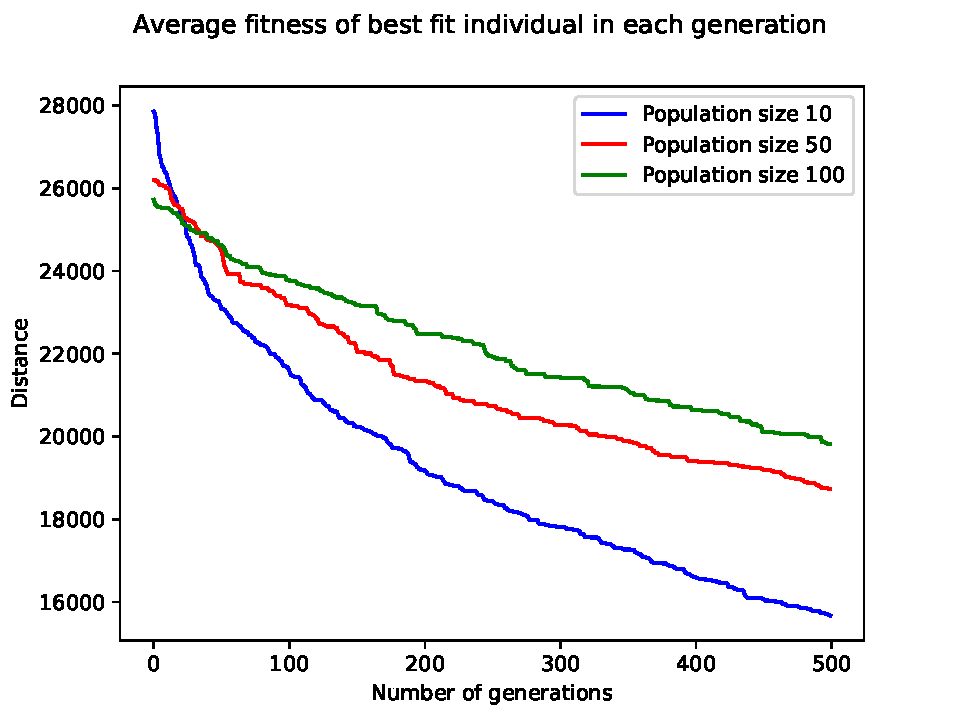
\includegraphics[scale=0.8]{"../genetic_algorithm.pdf}
\caption{Average fitness result for the genetic algorithm}
\end{center}
\end{figure}

\section{Hybrid algorithm}
Use hill climber on each individual as part of the evaluation, report min max mean deviation and average fitness with both Lamarckian and Baldwinian learning models, Compare result with GA
\subsection{Lamarckian learning model}
\begin{lstlisting}[language=bash]
---- LAMARCKIAN LEARNING MODEL ----
Search: 24 cities, population size: 10, number of generations: 500, 
number of rounds: 20, number of children: 4,number of hill climb iterations: 3: 
Best distance: 12416.869999999999
Worst distance: 14093.089999999998
Average distance: 13252.1
Standard deviation: 450.395
Time [seconds]: 17.240872
Best order of travel: 
Bucharest Istanbul Sofia Belgrade Budapest Vienna Milan Rome Barcelona 
Madrid Paris Brussels Munich Prague Berlin Hamburg London Dublin Copenhagen 
Stockholm Saint Petersburg Moscow Kiev Bucharest
 
Search: 24 cities, population size: 50, number of generations: 500, 
number of rounds: 20, number of children: 4, number of hill climb iterations: 3: 
Best distance: 12325.93
Worst distance: 13547.129999999997
Average distance: 12939.1
Standard deviation: 331.192
Time [seconds]: 71.480543
Best order of travel: 
Dublin London Paris Brussels Hamburg Prague Vienna Budapest Belgrade Sofia 
Istanbul Bucharest Berlin Copenhagen Stockholm Saint Petersburg Moscow Kiev 
Warsaw Munich Milan Rome Barcelona Dublin
 
Search: 24 cities, population size: 100, number of generations: 500, 
number of rounds: 20, number of children: 4 number of hill climb iterations: 3: 
Best distance: 12520.170000000002
Worst distance: 13455.670000000002
Average distance: 12983.2
Standard deviation: 254.007
Time [seconds]: 140.06269
Best order of travel: 
Copenhagen Stockholm Saint Petersburg Moscow Kiev Warsaw Budapest Bucharest 
Istanbul Sofia Belgrade Vienna Munich Milan Rome Barcelona Madrid Dublin 
London Paris Brussels Prague Berlin Copenhagen
 
Search: 10 cities, population size: 10, number of generations: 500, 
number of rounds: 20, number of children: 4 number of hill climb iterations: 3: 
Best distance: 7486.309999999999
Worst distance: 7486.31
Average distance: 7486.31
Standard deviation: 5.85938e-05
Time [seconds]: 9.794478
Best order of travel: 
Istanbul Bucharest Budapest Berlin Copenhagen Hamburg Brussels Dublin Barcelona 
Istanbul
 
Search: 10 cities, population size: 50, number of generations: 500, 
number of rounds: 20, number of children: 4 number of hill climb iterations: 3: 
Best distance: 7486.309999999999
Worst distance: 7486.3099999999995
Average distance: 7486.31
Standard deviation: 5.85938e-05
Time [seconds]: 40.547498
Best order of travel: 
Brussels Dublin Barcelona Belgrade Istanbul Bucharest Budapest Berlin Copenhagen 
Brussels
 
Search: 10 cities, population size: 100, number of generations: 500, 
number of rounds: 20, number of children: 4 number of hill climb iterations: 3: 
Best distance: 7486.309999999999
Worst distance: 7486.3099999999995
Average distance: 7486.31
Standard deviation: 5.85938e-05
Time [seconds]: 79.250088
Best order of travel: 
Budapest Bucharest Istanbul Belgrade Barcelona Dublin Brussels Hamburg Copenhagen 
Budapest
\end{lstlisting}

\begin{figure}[H]
\begin{center}
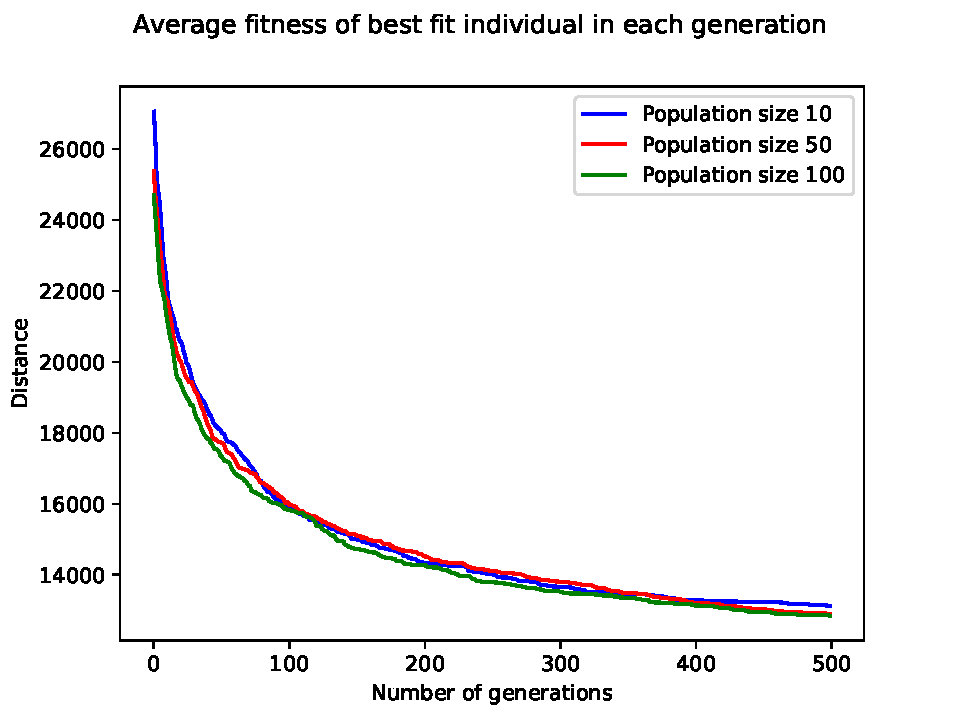
\includegraphics[scale=0.8]{"../hybrid_algorithm_lamarckian.pdf}
\caption{Average fitness result for the hybrid algorithm with a Lamarckian learning model}
\end{center}
\end{figure}

\subsection{Baldwinian learning model}
\begin{lstlisting}[language=bash]
---- BALDWINIAN LEARNING MODEL ----
Search: 24 cities, population size: 10, number of generations: 500, 
number of rounds: 20, number of children: 4 number of hill climb iterations: 3: 
Best distance: 23569.699999999997
Worst distance: 30698.32
Average distance: 27057.8
Standard deviation: 1698.52
Time [seconds]: 19.73016
Best order of travel: 
Paris Sofia Istanbul Bucharest Warsaw Dublin Berlin Belgrade Moscow Kiev Saint 
Petersburg Stockholm Vienna Milan Budapest London Brussels Copenhagen Madrid 
Rome Munich Barcelona Hamburg Paris
 
Search: 24 cities, population size: 50, number of generations: 500, 
number of rounds: 20, number of children: 4 number of hill climb iterations: 3: 
Best distance: 23313.62
Worst distance: 33411.56
Average distance: 27435.2
Standard deviation: 2288.74
Time [seconds]: 89.600072
Best order of travel: 
Vienna Belgrade Hamburg Copenhagen Stockholm Saint Petersburg Moscow Milan Kiev 
Berlin Prague Brussels Sofia Barcelona Warsaw London Dublin Paris Budapest 
Bucharest Istanbul Rome Madrid Vienna
 
Search: 24 cities, population size: 100, number of generations: 500, 
number of rounds: 20, number of children: 4 number of hill climb iterations: 3: 
Best distance: 24248.28
Worst distance: 31721.629999999994
Average distance: 27034.7
Standard deviation: 2062.25
Time [seconds]: 188.508705
Best order of travel: 
Hamburg Prague Saint Petersburg Moscow Belgrade Copenhagen Berlin Paris Brussels 
Milan Vienna Warsaw Rome Dublin London Stockholm Budapest Istanbul Kiev Barcelona 
Madrid Sofia Bucharest Hamburg
 
Search: 10 cities, population size: 10, number of generations: 500, 
number of rounds: 20, number of children: 4 number of hill climb iterations: 3: 
Best distance: 8612.61
Worst distance: 15709.300000000001
Average distance: 11665.6
Standard deviation: 2025.71
Time [seconds]: 14.102291
Best order of travel: 
Budapest Belgrade Istanbul Barcelona Hamburg Brussels Copenhagen Dublin Berlin 
Budapest
 
Search: 10 cities, population size: 50, number of generations: 500, 
number of rounds: 20, number of children: 4 number of hill climb iterations: 3: 
Best distance: 8312.79
Worst distance: 12810.14
Average distance: 10222.6
Standard deviation: 1503.26
Time [seconds]: 51.040574
Best order of travel: 
Belgrade Bucharest Dublin Copenhagen Berlin Budapest Hamburg Brussels Barcelona 
Belgrade
 
Search: 10 cities, population size: 100, number of generations: 500, 
number of rounds: 20, number of children: 4 number of hill climb iterations: 3: 
Best distance: 8450.56
Worst distance: 15331.689999999999
Average distance: 11454.8
Standard deviation: 1912.34
Time [seconds]: 99.088864
Best order of travel: 
Bucharest Copenhagen Hamburg Berlin Brussels Dublin Budapest Barcelona Belgrade 
Bucharest

\end{lstlisting}

\begin{figure}[H]
\begin{center}
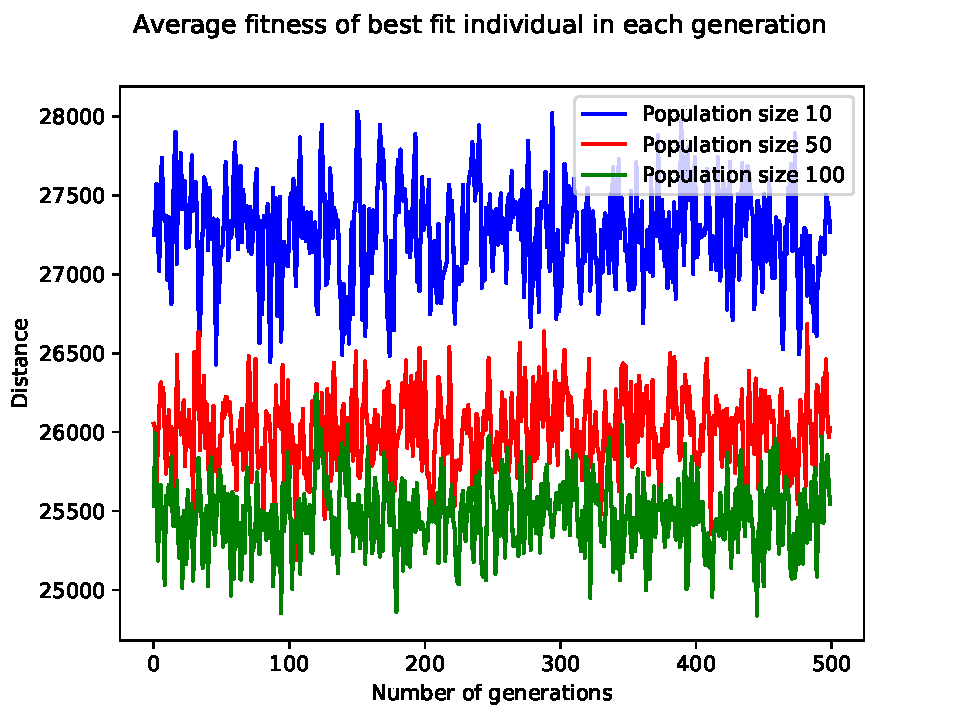
\includegraphics[scale=0.8]{"../hybrid_algorithm_baldwinian.pdf}
\caption{Average fitness result for the hybrid algorithm with a Baldwinian learning model}
\end{center}
\end{figure}

\end{document}
